\documentclass{article}
\usepackage{tikz}

\begin{document}

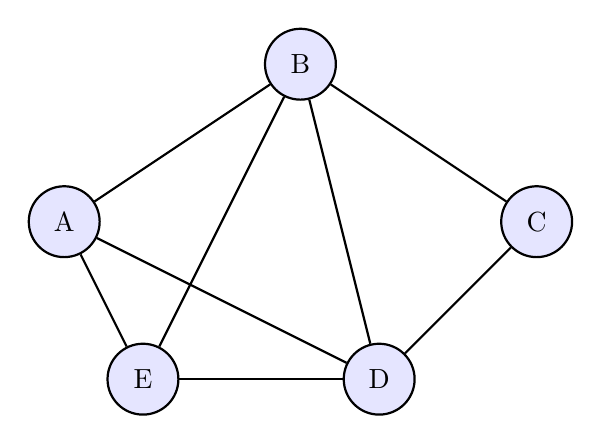
\begin{tikzpicture}[
    vertex/.style={
        circle,
        draw,
        thick,
        minimum size=9mm,
        fill=blue!10
    }
]

    % Vertices
    \node[vertex] (A) at (0,2) {A};
    \node[vertex] (B) at (3,4) {B};
    \node[vertex] (C) at (6,2) {C};
    \node[vertex] (D) at (4,0) {D};
    \node[vertex] (E) at (1,0) {E};

    % Edges
    \draw[thick] (A) -- (B);
    \draw[thick] (B) -- (C);
    \draw[thick] (C) -- (D);
    \draw[thick] (D) -- (E);
    \draw[thick] (E) -- (A);

    % Diagonal edges
    \draw[thick] (A) -- (D);
    \draw[thick] (B) -- (D);
    \draw[thick] (B) -- (E);

\end{tikzpicture}

\end{document}
